\documentclass[main.tex]{subfiles}
\begin{document}
\onlyinsubfile{\mainmatter{}}

\chapter{Glyco Heap-based Secure Calling Convention} \label{ch:ghscc}
The previous chapter discusses the first milestone of the Glyco compiler, namely a nanopass compiler producing fairly traditional executables for CHERI-RISC-V targets, with almost no special considerations for capability machines, except for minor enhancements such as bounded heap-allocated buffers. This chapter explores the first significant upgrade of the Glyco compiler, namely one where procedure calls are implemented using a secure \g{cc} named \textbf{\g{ghscc}} and adapted from the heap-based \g{cc} proposed by \citet{cerise}.

We first describe in \cref{sct:scc} the desired security properties of a \enquote{secure} \g{cc}. We then detail in \cref{sct:ghscc-rt} the low-level implementation of two \gs{rtrt} that form the basis of \g{ghscc}. After that, we explore in \cref{sct:ghscc} the implementation of the \g{cc} itself. We then evaluate in \cref{sct:ghscc-eval} \g{ghscc} against \g{gccc} in terms of changes to the compiler and its \gs{il}, generated codesize, and runtime performance. We finish in \cref{sct:alt-scc} by listing a few alternative secure \gs{cc} that are either already implemented or did not make it into Glyco.

This chapter discusses the feature set and languages of Glyco 0.2,\footnote{The source code is available at \url{https://tsarouhas.eu/glyco/0.2/}.} however just like in the previous chapter, example programs in this chapter follow the syntax of the final version of the compiler, Glyco 1.0. A full language reference of this final compiler can be found in \cref{ch:grammar}.

\section{Background: Secure Calling Conventions} \label{sct:scc}
A traditional \g{cc} such as \g{gccc} works with a single stack of call frames per thread, with each call frame holding a procedure call's ephemeral state, such as values assigned to local variables. When a procedure is called, a new call frame is pushed on the stack, the caller puts a return address in a designated register or location on the call frame, and passes control to the callee. When returning, the most recent call frame on the stack is popped and the callee jumps to the caller-provided return address. The exact details and distribution of responsibilities are mandated by the \g{cc} in use.

A traditional \g{cc} however provides no security in the face of adversarial code that operates in the same address space. For one, adversarial code has access to the full call stack and thus to other call frames than its own. The adversarial code may be from an external dependency that has not been rigorously vetted, but it may also be first-party code containing an overflow vulnerability on a statically-allocated buffer that is exploited with specially crafted input, as illustrated in \cref{fig:buffoverflow}. \textbf{\Gls{lse}} is a security property that makes it \textbf{impossible for a procedure to access the local state,} i.e., call frame, \textbf{of another procedure,} or for a procedure in one compartment (such as a library) to access the local state of a procedure in another compartment.

\begin{SCfigure}
	\centering
	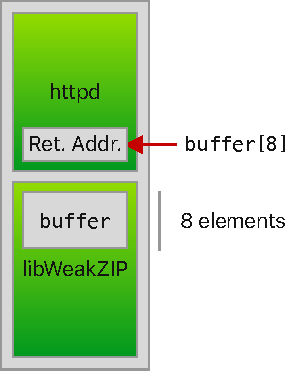
\includegraphics{Images/Buffer Overflow.pdf}
	\caption{A vulnerability in a (trusted) libWeakZIP procedure may allow an attacker to overflow the stack-allocated buffer. In this example, the return address is stored at the end of the caller's call frame and is thus overwritten by the attack. Note that the stack grows downward.}
	\label{fig:buffoverflow}
\end{SCfigure}

A different but related problem is that adversarial code may ignore the \g{retcap} provided by the caller and instead return to a different location, within or outside the caller. They may, for instance, skip an authentication check by jumping straight into the execution path of a successful authentication, or they might return to the caller's caller as illustrated in \cref{fig:no-wbcf}. They may also store the provided \g{retcap} and jump to it more than once. In contrast when \textbf{\g{wbcf}} applies, \textbf{a procedure can only call procedures, return to its caller, or diverge} (e.g., get stuck in an infinite loop).

\begin{SCfigure}[][ht]
	\centering
	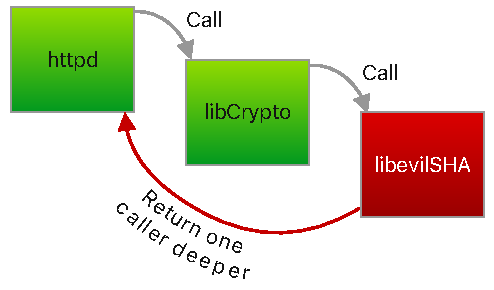
\includegraphics{Images/No WBCF.pdf}
	\caption{An example demonstrating one kind of attack when \g{wbcf} is not guaranteed. libevilSHA returns one caller deeper, skipping libCrypto and leaving it waiting to be returned to.}
	\label{fig:no-wbcf}
\end{SCfigure}

A \g{cc} proposed by \citet[section~7.3]{cerise} provides \g{lse} by ensuring that call frames always occupy freshly allocated memory to which certainly no dangling capabilities point. However it does not provide \g{wbcf}. \g{ghscc} adapts a variant of this \g{cc} that provides \g{lse} and a weaker variant of \g{wbcf}.

\section{Secure Heap Allocation \& A Runtime} \label{sct:ghscc-rt}
As the name suggests, \acrlong{ghscc} uses the heap instead of a call stack. A secure implementation of \g{ghscc} depends on a secure implementation of heap allocation as described by \citet[section~7.1]{cerise}: a region of memory belonging to a heap-allocated buffer must only be accessible to \gs{userp} via the capability provided by the allocator when that buffer is allocated.

Glyco implements a simple \emph{bump-pointer} allocator where an allocation is performed by returning an appropriately bounded capability to the first free region in heap memory and offsetting an internal \textbf{\g{heapcap}} to point to the next free location after the allocated buffer. Deallocation is not supported; the allocator therefore never returns a capability to a region of memory used by a previously allocated buffer.\footnote{As described by \citet[section~2.3.16]{cheri}, capability revocation in a garbage-collected system can be implemented in several ways such as scanning accessible memory to revoke dangling capabilities, or having the memory management unit prevent accesses to deallocated buffers. Revocation and garbage collection are outside this thesis' scope.}

To implement heap allocation and future functionality securely, Glyco is extended with support for \gs{rtrt}, which are procedures provided by the language \g{rt}, with capabilities not afforded to normal procedures, and possibly using a different (often more basic) \g{cc} than ordinary procedures. Each \g{rtrt} is stored in memory not directly accessible to \gs{userp} except via a \g{sentry} to the routine's entry point, as can be seen in \cref{fig:procmem}.

\begin{figure}
	\centering
	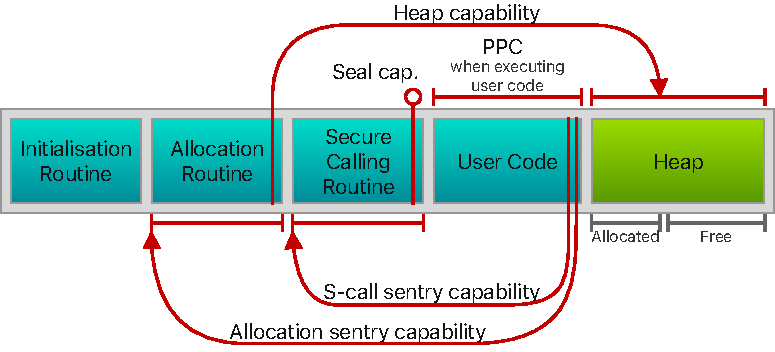
\includegraphics{Images/GHSCC Process Memory.pdf}
	\caption{The process memory layout of a program compiled with \g{ghscc}. The allocation routine contains a \g{heapcap} that grants access to the heap and points to the next allocatable location in it. The secure calling routine embeds a \g{sealcap} which it uses to seal the \texttt{cra}–\texttt{cfp} pair for callees. Both routines are accessible to the \g{userp} only via a \g{sentry}.}
	\label{fig:procmem}
\end{figure}

As Glyco is developed almost entirely in isolation, it cannot rely on an operating system or dynamic linker to provide these routines and therefore provides them itself. It is expected that a production compiler would be able to rely on an OS-provided standard library instead, thereby removing the need to trust the compiler and its \g{rt}.

The first \g{rtrt} is a \textbf{heap allocation routine}, which accepts a byte size in \texttt{t0} and a \g{retcap} in \texttt{ct2} and returns a unique capability to an allocated buffer in \texttt{ct1}. The \g{heapcap}, providing access to the full heap and pointing to the next free location in it, is stored within the allocator's memory. This ensures that, at any point in time, only the allocator has access to unallocated memory and that memory associated with an allocated buffer is only ever accessible to the allocator and whoever holds the capability to that buffer returned by the allocator.
\todo{Add assembly excerpt of heap allocation routine.}

\section{Call Frame Encapsulation \& Secure Calling} \label{sct:ghscc}
A procedure allocates a buffer for its call frame in its prologue by calling the heap allocation routine with an appropriate byte size, and uses the call frame just as it would with \g{gccc}. The heap allocation routine ensures that only it and the procedure have access to the buffer,\footnote{The \g{rt} is implicitly trusted in our threat model. In a realistic compiler and runtime environment with a heap allocation routine, the program would need to trust at least the dynamic linker and any linked runtime code.} thereby ensuring that \g{lse} holds at that point in time.

A procedure call in \g{ghscc} is realised using a \textbf{secure calling (s-call) routine} and is therefore referred to as an \textbf{\g{scall}}. This \g{rtrt} expects a target capability in \texttt{ct6}, a \g{retcap} in \texttt{cra}, and a \g{framecap} in \texttt{cfp}. When invoked, the routine generates a unique \g{sealcap}, seals the frame and return capabilities, and jumps to the target capability's address. Similar to how the heap capability in the allocation routine grants the latter access to the heap and points to the next free location, the \g{scall} routine contains a \g{sealcap} that grants it \g{sealing} power for all \gs{otype} and whose address is the next available \g{otype}. \todo{Add assembly excerpt of \g{scall} routine.} An \g{scall} looks as follows:

\begin{enumerate}
	
	\item Just as with \g{gccc}, the caller puts the arguments for the callee in argument registers. However, if there are more parameters than there are argument registers, an arguments record is allocated on the heap (using the \g{rtrt} described above), a capability to it is put in the last argument register, and any arguments that do not fit in registers are stored in the arguments record. The callee never needs to access the caller's call frame to gain access to arguments that did not fit in registers, nor does the caller need access to the callee's call frame to store supplementary arguments.
	
	\item \label{itm:returned-init} The caller initialises a value \texttt{returned} to 0 and stores it in its call frame. This value is later used to protect against multiple uses of the \g{retcap}.
	
	\item The caller clears all registers except those used for the \g{framecap} and for arguments. This ensures that the callee does not accidentally receive any authority beyond what is explicitly passed to it.
	
	\item The caller invokes the \g{scall} routine, passing to it a target capability to the caller and a \g{retcap} to itself. The routine also receives the caller's \g{framecap} via \texttt{cfp}.
	
	\item The routine seals the received \g{framecap} and \g{retcap} with its \g{sealcap}, then increases the \g{sealcap}'s address to ensure that the next \g{scall} is sealed with a unique \g{otype}.
	
	\item The routine clears any registers that it has used itself to ensure it does not accidentally leak new authority, then jumps to the target capability's address (the callee).
	
	\item The callee allocates a call frame using the heap allocation routine. It then stores the caller's (sealed) \g{framecap} in its new call frame, unless the callee is a leaf procedure, i.e., unless it calls other procedures.\footnote{This behaviour emerges from the fact that the register allocator spills the locations containing the caller's sealed frame and return capabilities when a procedure contains a call effect.}
	
	\item The callee executes its effect.
	
	\item When the callee is done, it clears all registers except those used for the result and the \g{retcap}. This ensures that the caller does not accidentally receive any authority beyond what is explicitly returned to it.
	
	\item The callee returns control to the caller with \hbox{\texttt{cinvoke cra, cfp}} where \texttt{cra} and \texttt{cfp} are the return resp. frame capabilities provided to the callee by the \g{scall} routine. The machine unseals the two capabilities after checking that they have the same \g{otype} and that they comply with the instruction's preconditions,\footnote{Among these preconditions are: the first operand must be valid and executable and the second operand must be valid and nonexecutable.} then puts the second operand (\texttt{cfp}) in \texttt{ct6}, and finally jumps to the first operand's address (\texttt{cra}).
	
	\item The caller restores its \g{framecap} by moving the capability in \texttt{ct6} back to \texttt{cfp}.
	
	\item The caller checks whether \texttt{returned} from Step~\ref{itm:returned-init} is equal to 0. If it is, it is set to 1; otherwise, the program crashes by attempting to load a value using the null capability.
	
	\item The caller resumes execution.
	
\end{enumerate}
\todo{Add \g{nanopass} example.}

As part of an \g{scall}, the callee receives arguments and a return–frame capability pair sealed with a unique \g{otype} for which the callee has no \g{unsealcap} and therefore cannot dereference. The callee thus cannot access the caller's local state, thereby preserving \g{lse}. The capabilities are only unsealed when control is returned to the caller using the atomic \texttt{CInvoke} instruction. Since the callee also does not have a \g{sealcap} for that \g{otype}, it cannot forge a call stack to manipulate the procedure's local state, nor can it forge a \g{retcap} to trick \texttt{CInvoke} into unsealing the sealed \g{framecap} before invoking adversarial code.

Before invoking the \g{scall} routine, the caller initialises an indicator value to 0 and stores it in its call frame. When the callee returns control to the caller, the caller checks if the value is still 0 and crashes otherwise. It then sets the value to 1 to ensure that subsequent uses of the \g{retcap} result in a machine trap, thereby ensuring that the \g{retcap} is only usable once. Since \g{lse} protects the call frame from external access, it also protects the indicator value from the same.

The latter security property, which we call \textbf{unrepeatable return}, is a weaker variant of \g{wbcf} and can be stated as follows: \textbf{a \g{retcap} provided by a procedure supporting unrepeatable return can be used at most once}. Unlike \g{wbcf}, it does not disallow a callee to return to another procedure's caller, as illustrated in \cref{fig:semi-wbcf}.

\begin{figure}
	\centering
	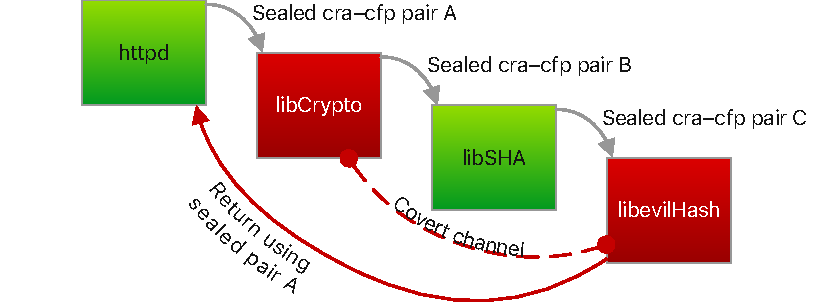
\includegraphics{Images/Semi-WBCF.pdf}
	\caption{\G{ghscc} does not support \g{wbcf}. In this example, libCrypto sends the return–frame capability pair it receives from httpd to libevilHash, which uses it to return directly to httpd, thereby leaving libSHA (and libCrypto) waiting to be returned to.}
	\label{fig:semi-wbcf}
\end{figure}

\section{Evaluation} \label{sct:ghscc-eval}
\subsection{Impact on the Codebase}
We now evaluate the impact of the implementation of \g{ghscc} in Glyco which can serve as an indicator to the development effort required for adding a new \g{cc} to an existing \g{nanopass} compiler with a similar design. We first present the most significant changes to Glyco's languages, going from low-level to high-level \gs{il}, then quantify the codebase's growth. The changes to the compiler pipeline are also summarised in \cref{fig:pipeline02}.

\begin{figure}
	\centering
	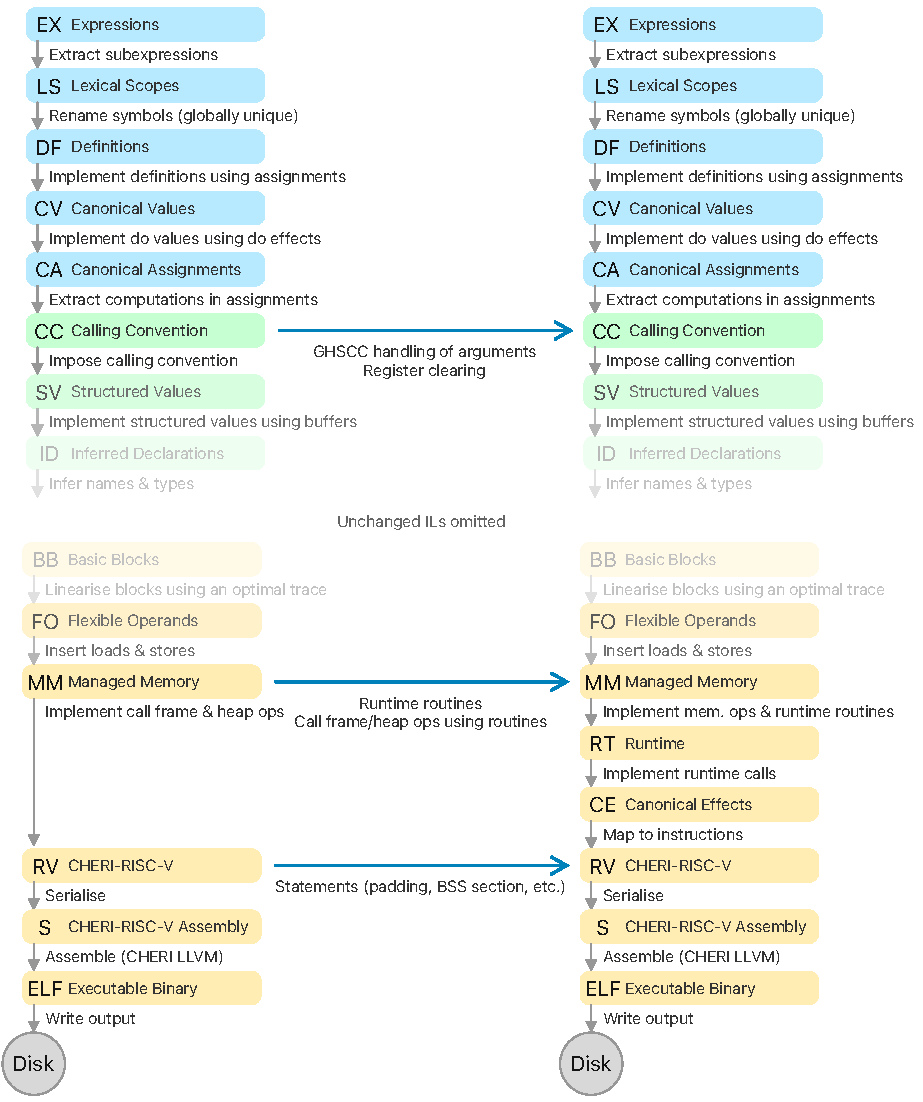
\includegraphics{Images/Pipeline v0.2.pdf}
	\caption{The Glyco 0.1 (left) and 0.2 (right) pipelines and the main differences between them.}
	\label{fig:pipeline02}
\end{figure}

\paragraph{CHERI-RISC-V (RV)} The low-level language RV is extended with additional grammar for statements such as \texttt{padding} and \texttt{bssSection}, which can be \glslink{lowering}{lowered} trivially to their CHERI-RISC-V assembly counterparts. Instructions are now merely one kind of statement, and programs are redefined as a list of statements. This additional grammar is required by MM which now explicitly manages regions of memory for use by the call stack, the heap, or \gs{rtrt}.

\paragraph{Canonical Effects (CE)} To avoid overloading MM's \g{nanopass} with responsibilities, a new \g{il} is defined above RV grouping related instructions. Instructions such as \texttt{copyWord} and \texttt{copyCapability} are for instance exposed under a single \texttt{copy} effect in CE, which MM inherits.

\paragraph{Runtime (RT)} To facilitate calling \gs{rtrt} (which behave differently than ordinary procedures), a new \g{il} RT is defined above CE providing a \texttt{callRuntimeRoutine} effect. This effect accepts a label to a capability located in memory accessible to the \g{userp}, loads the capability, and jumps to its address. These capabilities are \gs{sentry} to \g{rt} memory; \gs{userp} cannot dereference these capabilities but they can jump to their address. This prevents a \g{userp} from accessing the \g{rt}'s internal data structures like the \g{heapcap}.

\paragraph{Managed Memory (MM)} MM moves above RT but its grammar remains mostly the same as in the previous version. The MM (to RT) \g{nanopass} however changes significantly. When a \texttt{Program} is \lowered{}, MM now includes runtime initialisation code, explicit ELF sections for the call stack and heap, and \gs{sentry} to the allocation and \g{scall} \gs{rtrt}. The \g{lowering} of the \texttt{createBuffer} effect is updated to invoke the allocation routine instead of directly manipulating the heap capability (previously kept in register \texttt{ctp}). The \texttt{pushFrame} effect now allocates a call frame on the heap.

\paragraph{Calling Convention (CC)} The \texttt{call} effect in CC is updated to allocate an arguments record for arguments that do not fit in the available argument registers, and to clear registers before calling the procedure.

\paragraph{Codebase growth} The implementation of \g{ghscc} introduces 2 new \gs{il} (RT and CC) bringing the total in Glyco 0.2 to 19 \gs{il}. Using cloc,\footnote{cloc is available at \url{https://github.com/AlDanial/cloc}.} we measured a growth in the codebase from 5941 SLOC in Glyco 0.1 to 6921 SLOC in Glyco 0.2, representing a net growth of $+16\%$.\footnote{The source line of code metric (SLOC) excludes empty lines and comments but does not perform other normalisation. For instance, multiple statements on a single line still count as 1 SLOC.}

The compiler's implementation does not rely on a framework such as one described by \citet{commcomp} that provides a compact syntax for deriving a new \g{il} given an existing \g{il}.\footnote{On the other hand, the Swift compiler assists the developer with its type checker, pattern exhaustiveness checker (for ensuring all syntax patterns are handled in \gs{nanopass}), and automatic conformance to protocols such as \texttt{Equatable} or \texttt{Codable} which are used for testing and representing programs as Sisp values.} New \gs{il} are instead derived by duplicating parts of the \g{lowerlang}'s source files and adapting them for the new \g{il}. The SLOC metric is therefore not as informative as the number of added \gs{il} or changes per \g{il}.

\subsection{Impact on Build Products}
We now evaluate \g{ghscc} itself by benchmarking a few test programs against the previous \g{cc}.

\paragraph{Increased binary footprint} For measuring the binary footprint, we decided to measure the number of statements and instructions in the assembly of a few test programs as opposed to measuring the byte size of the executables themselves. The latter metric is less informative since the space taken up by ELF headers and structures dominates the space occupied by the code of interest.

The test programs are compiled in Glyco 0.2 using a default configuration targeting the CHERI-RISC-V Sail emulator and using the \g{gccc} and \g{ghscc} \gs{cc}. The default configuration enables all optimisations provided by Glyco.

The minimalistic test program 42 immediately evaluates to the number 42. The fib test program computes the 30th or 300th number of the Fibonacci sequence using a recursive function with accumulator parameters to avoid redundant computations. The Euclid test program computes the greatest common divisor of 20 and 50 or of 441 and 520 using a simple subtraction algorithm. As shown in \cref{tbl:ghscc-size}, a visible increase in binary footprint can be observed.

\begin{table}[h]
	\medskip	% fixes glitch where heading seems vertically compressed
	\begin{adjustwidth}{-1in}{-1in}
		\centering
		\footnotesize
		\begin{tabular}{ccccccccccc}
			\toprule
								& \multicolumn{4}{c}{\g{gccc}}			& \multicolumn{3}{c}{\g{ghscc}}		& \multicolumn{3}{c}{$\Delta$}		\\
								\cmidrule(lr){2-5}						\cmidrule(lr){6-8}					\cmidrule(lr){9-11}
			Program				& Size	& Time		& Stack		& Heap	& Size	& Time		& Heap		& Size		& Time		& S + H		\\
			\midrule
			Runtime				& 75	& —			& —			& —		& 110	& —			& —			& $+47\%$	& —			& —			\\
			\addlinespace
			42					& 45	& 107 t		& 32 B		& 0 B	& 66	& 207 t		& 96 B		& $+47\%$	& $+93\%$	& $+200\%$	\\
			fib(0, 1, 30)		& 53	& 705 t		& 1.50 kB	& 0 B	& 114	& 2.41 kt	& 2.51 kB	& $+115\%$	& $+241\%$	& $+67\%$	\\
			fib(0, 1, 300)		& 53	& 1.61 kt	& 14.4 kB	& 0 B	& 114	& 22.1 kt	& 15.4 kB	& $+115\%$	& $+1278\%$	& $+7\%$	\\
			Euclid(20, 50)		& 62	& 170 t		& 208 B		& 0 B	& 151	& 441 t		& 1.36 kB	& $+144\%$	& $+159\%$	& $+554\%$	\\
			Euclid(441, 520)	& 62	& 478 t		& 880 B		& 0 B	& 151	& 1.49 kt	& 2.08 kB	& $+144\%$	& $+212\%$	& $+136\%$	\\
			\bottomrule
		\end{tabular}
	\end{adjustwidth}
	\caption{Benchmarking test programs in \g{gccc} and \g{ghscc} in Glyco 0.2. The program size is measured in number of assembly statements and is split between the runtime and the rest of the program. Time is measured in ticks (or kiloticks), with one instruction being executed per tick. Stack and heap sizes are maxima.}
	\label{tbl:ghscc-size}
\end{table}

\paragraph{Increased runtime and memory overhead} For measuring runtime overhead, the same test programs are executed in the CHERI-RISC-V Sail emulator and the number of steps to completion is counted. For memory overhead, the distance between the highest and lowest address of the \g{stackcap} and \g{heapcap} (after runtime initialisation) is determined. As shown in \cref{tbl:ghscc-size}, a significant degradation in performance can be observed when using \g{ghscc} in a function call-heavy program.

\todo{Add test program that always allocates something on the heap.}

\section{Related Work: Alternative Secure Calling Conventions} \label{sct:alt-scc}
The heap-based \g{cc} proposed in this chapter and implemented in Glyco is but one \g{cc} providing \g{lse}, albeit without a rigorous proof. Several alternatives have been proposed in literature or are implemented in CHERI software, some of which also provide \g{wbcf}.

To ensure \g{lse} with a stack-based \g{cc}, a caller can restrict the \g{stackcap} before calling a procedure so that the callee only gets access to the unused part of the stack. However, this approach requires a way for the caller to restore the previous (less restricted) \g{stackcap} without the callee being able to do the same. Additionally, as illustrated in \cref{fig:savedstackcap}, an adversary can save a copy of their (restricted) \g{stackcap} in a first call. If the adversary is called a second time when their \g{stackcap} is lower in the stack (due to the stack containing more call frames than during the first call), it can use the saved \g{stackcap} to gain access to memory used by other call frames. They can similarly store the \g{retcap} and use it more than once, breaking \g{wbcf}.

\begin{figure}
	\centering
	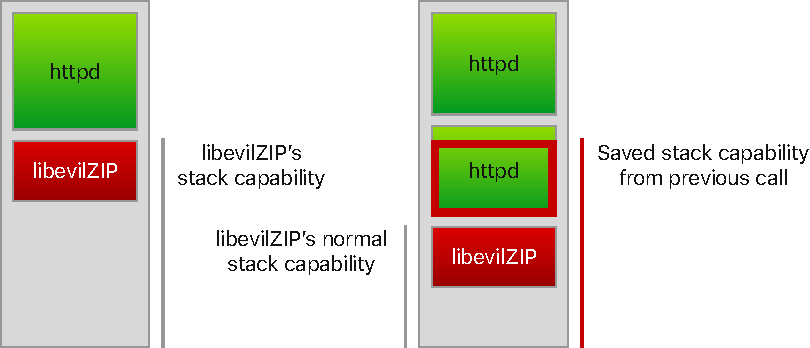
\includegraphics{Images/Saved Stack Cap.pdf}
	\caption{The call stack in a first invocation (left) and a second invocation (right) of the adversary, where the second invocation's call frame is at a lower address than the first invocation's call frame. During the first invocation, the adversary saves their \g{stackcap} for use during a later invocation. Even though the \g{stackcap} in the second invocation provides authority over a smaller part of the call stack, the previously saved \g{stackcap} continues to provide the adversary with authority over the larger region, which now includes memory occupied by other call frames. Note that the stack grows downward.}
	\label{fig:savedstackcap}
\end{figure}

\paragraph{Using local capabilities to revoke copies of the \g{stackcap}} A \g{cc} proposed by \citet{retptr} relies on \textbf{local capabilities}, a type of capability that can be only kept in registers and stored using capabilities that allow storing local capabilities. Local capabilities in CHERI are capabilities without the \emph{Global} permission, whereas capabilities that can be used to store local capabilities have the \emph{Store local capability} permission.

Just before a procedure is called, the caller pushes a restoration routine\footnote{\citet{retptr} uses the term \emph{activation record} instead, but since it's commonly also a synonym for \emph{call frame}, we decided against reusing this terminology in this thesis.} on the call stack, sets the \g{retcap} to point to that restoration routine, and seals it as a \g{sentry}. The restoration routine restores the caller's \g{stackcap} and returns to the caller; the saved stack and return capabilities used by the routine are therein embedded.

To prevent the callee from saving their return and stack capabilities somewhere, the two capabilities are marked as local. However, they still need to be saved in the restoration routine. Since this routine is part of the call stack, the \g{stackcap} is given the \emph{Store local capability} permission. This permission is not given to capabilities to any other region of memory, ensuring that return and stack capabilities cannot be saved elsewhere. Since the adversary can still save these capabilities somewhere in stack memory, e.g., far from any call frames where it's unlikely to be overwritten, the unoccupied part of the stack must be cleared before calling or returning to a possible adversary.

The \g{cc} guarantees both \g{lse} and \g{wbcf} since an adversary cannot retain either a stack or return capability after it returns. However, it requires clearing of potentially large regions of unoccupied stack memory which is inefficient if no hardware support is available. Furthermore, since the call stack needs to hold executable restoration routines, the \g{stackcap} needs the \emph{Permit execute} permission, and thus special care must be taken to avoid accidentally executing code stored in input buffers.

Even though this \g{cc}'s security properties have been proven using a mechanised proof, we did not consider implementing this \g{cc} in Glyco because no emulator supports efficient stack clearing and manual stack clearing would dominate the test programs' runtime.

\paragraph{Using local uninitialised capabilities to revoke copies of the \g{stackcap}} A \g{cc} proposed by \citet{uninitcapss,uninitcaps} builds on the aforementioned \g{cc} but removes the requirement for clearing large regions of stack memory. It instead relies on \textbf{uninitialised capabilities}, a type of capability proposed by \citet{uninitcapss} only allowing loads on an initialised part of its bounds. Storing a datum immediately after the initialised region extends the capability's initialised region to include the newly stored datum.

In this \g{cc}, the restoration routine still restores the caller's \g{stackcap} except that the \g{stackcap} is now an uninitialised capability. This saved \g{stackcap} has a smaller initialised region, effectively revoking access to the unoccupied stack memory's contents. The next procedure called by this procedure will need to overwrite any unoccupied stack memory before accessing it.

A callee still needs to clear the stack memory occupied by their own call frame before returning to a potential adversary since the caller may have prepared a separate \g{stackcap} granting it access to the callee's call frame.\footnote{The caller still has a call frame where it can validly store any local capability.} However, the memory occupied by a single call frame is orders of magnitude smaller than the full unoccupied stack memory that needs to be otherwise cleared at every call or return.

Similarly to the previous \g{cc}, it is rigorously proven for an abstract machine with local and uninitialised capabilities. Uninitialised capabilities are however as of writing not fully specified for CHERI-RISC-V in an authoritative document such as by \citet{cheri}.

\paragraph{Using linear capabilities to restrict copies of the \g{stackcap}} The \emph{StkTokens} \g{cc} by \citet{stktokens} relies on \textbf{linear capabilities}, a type of capability that can only be moved, not copied. Before calling a procedure, the caller performs a splitting operation which splits the \g{stackcap} into two disjoint capabilities. The \g{stackcap} over the caller's call frame as well as the callee's \g{retcap} are sealed together with a unique \g{sealcap}. The caller then hands the sealed pair as well as the second (still unsealed) \g{stackcap} over to the callee.

The callee returns control to the caller by passing the unsealed \g{stackcap} to the caller (e.g., via the dedicated \g{stackcap} register) and invoking the sealed stack–return capability pair. The machine unseals both capabilities and jumps to the caller. The caller merges the two \gs{stackcap} back to get its original \g{stackcap}, over both its call frame and the unused part of the stack.

\G{lse} is guaranteed by the \g{stackcap}'s linearity: the callee must yield its unsealed \g{stackcap} to the caller before the caller can reconstruct its previous \g{stackcap}. In addition, the callee only gets a sealed \g{stackcap} to the caller's call frame and thus is not granted access to the call frame, assuming the caller uses a unique \g{sealcap} that it does not hand to the callee.

\G{wbcf} is guaranteed by the \g{retcap}'s linearity: the callee can only return to the caller by invoking the stack–return capability pair, losing access to both capabilities in the process. The callee also cannot return to a caller deeper in the stack as that (deeper) caller is unable to reconstruct their \g{stackcap} without its callee's cooperation.

Although this \g{cc} is delightfully straightforward in its design, linear capabilities are as of writing not authoritatively specified for CHERI-RISC-V.

\paragraph{Using one call stack per compartment} As described by \citet{compartment}, CheriBSD supports compartmentalising software components (such as libraries) whereby each component gets its own call stack, with the operating system managing a central stack per thread. This approach however requires one call stack per component per thread, one central stack per thread, and one syscall per security domain transition, i.e., when a compartment's procedure calls or returns into another compartment's procedure. Furthermore, it does not provide complete \g{lse} since it only protects components from other components; a vulnerability in a procedure within a library may compromise all call frames from that library in the same thread. Similarly, \g{wbcf} across components can be enforced by the system since returns across components are mediated by the OS, but the property does not apply within a single component.

\biblio{}
\onlyinsubfile{\glsaddall\printglossaries}
\end{document}
